\documentclass[conference]{IEEEtran}
\usepackage[colorlinks=true,allcolors=blue,hypertexnames=false]{hyperref}
\usepackage{float}
\usepackage[table]{xcolor}
\usepackage{booktabs}
\usepackage{graphicx}
\definecolor{diagramblue}{HTML}{1D5CA1}

\begin{document}

\title{Email Classification for Financial Services}

\author{
    \IEEEauthorblockN{Msesenyane Makhongela}
    \IEEEauthorblockA{\href{mailto:khongela7@gmail.com}{khongela7@gmail.com}}
}

\maketitle

\setlength{\parindent}{0pt}
\setlength{\parskip}{0.5\baselineskip}

\section{Problem}
RedRock receives many client emails and needs to send each one to the right department. Sending an email to the wrong team could delay a response and create problems in a regulated financial business.

We are given 44 emails with known categories and 12 emails to classify. For each of the 12 emails, we need to choose one of five categories: Account Management, Investment Advisory, Loan Processing, Insurance Claims, or Other. The classifications need to be provided with a confidence score and saved in a CSV file.

In machine learning, this is a multiclass classification problem. A multiclass classifier chooses one category from a set of possible categories for each email. Here, the input is the email text and the output is one of the five business categories.

\section{Introduction}
There are several ways to solve this problem. We could turn the text into TF-IDF features and train a logistic regression model, use semantic embeddings, or ask a large language model to classify each email through an API. I began with the simpler approach so I could understand its decisions and test its performance on the labelled emails.

TF-IDF stands for term frequency inverse document frequency. It turns each email into numbers by giving more weight to words that appear often in that email but are less common across the training set.

Logistic regression learns how strongly those numbers are associated with each category and chooses the category with the highest predicted score. Multinomial Naive Bayes is another text classifier. It estimates how likely the words in an email are under each category and chooses the most likely category.

\section{Related Work}
I started by reading studies that compare ways to classify emails into several categories. Soni et al.~\cite{soni2024} studied organizational email sorting and found that logistic regression performed best when they combined TF-IDF and Word2Vec features. They also tested Multinomial Naive Bayes with TF-IDF. This study informed my initial thinking on model choice, while the results on RedRock's emails guided my final choice.

I also looked at two GitHub projects. avannaldas~\cite{avannaldas} used TF-IDF with an SGD classifier and grid search. VoxDroid~\cite{voxdroid} used word counts with Multinomial Naive Bayes. These examples helped me compare simple ways to classify email text.

\section{Methodology}

\subsection{Preparing the emails}
I used Beautiful Soup to extract each email's ID, subject and body from the supplied HTML files. I removed scripts and styles, then combined the subject and body into one text field for classification. I matched the training emails to their labels using filenames and kept the IDs from the HTML for the final results.

\subsection{Training the model}
I built a scikit-learn pipeline using TF-IDF and logistic regression. The vectorizer converted the email text into numerical features and removed common English stop words. During cross-validation, it learned its vocabulary only from the training emails, keeping the evaluation emails separate.

I used grid search to compare 12 combinations of single-word or word-pair features, regularization settings and class balancing. The settings with the highest average macro F1 were selected.

\subsection{Saving the predictions}
After evaluation, I fitted the tuned model using all 44 labelled emails and saved the pipeline. I used it to classify the 12 unlabelled emails, choosing the category with the highest predicted probability for each message. I exported the email IDs, predicted categories and confidence scores to a CSV file with the required column names.

\section{Evaluation and Results}

I used cross-validation to compare logistic regression, Multinomial Naive Bayes and an SGD classifier. I then tested different settings for the best classifier.

\begin{table}[H]
\centering
\footnotesize
\setlength{\tabcolsep}{6pt}
\renewcommand{\arraystretch}{1.0}
\caption{Cross-validation results for logistic regression.}
\label{tab:results}
\begin{tabular}{@{}lcc@{}}
\toprule
\rowcolor{diagramblue}
\textcolor{white}{Settings} &
\textcolor{white}{Accuracy} &
\textcolor{white}{Macro F1} \\
\midrule
\rowcolor{diagramblue!5}
Default settings & 79.09\% & 0.67 \\
\rowcolor{diagramblue!12}
Tuned settings & 92.73\% & 0.90 \\
\rowcolor{diagramblue!5}
Extra subject weighting & 91.36\% & 0.88 \\
\bottomrule
\end{tabular}
\end{table}

Which model worked best?

Logistic regression performed better than Multinomial Naive Bayes and SGD in the first comparison, so I used it for the remaining experiments.

Did tuning help?

Tuning improved the model, while giving more weight to the subject line did not. 

How trustworthy are the results?

The results are promising, but only 44 labelled emails were available. A larger test set is needed to confirm how well the model performs on new emails.

\begin{table}[H]
\centering
\footnotesize
\setlength{\tabcolsep}{3pt}
\renewcommand{\arraystretch}{1.0}
\caption{Predictions for the 12 unlabelled emails.}
\label{tab:predictions}
\begin{tabular}{@{}rlr@{}}
\toprule
\rowcolor{diagramblue}
\textcolor{white}{Email ID} & \textcolor{white}{Predicted category} & \textcolor{white}{Score} \\
\midrule
35 & Investment Advisory & 0.21 \\
\rowcolor{diagramblue!5}
2 & Investment Advisory & 0.23 \\
8 & Loan Processing & 0.24 \\
\rowcolor{diagramblue!5}
41 & Account Management & 0.22 \\
44 & Investment Advisory & 0.22 \\
\rowcolor{diagramblue!5}
7 & Investment Advisory & 0.22 \\
53 & Account Management & 0.22 \\
\rowcolor{diagramblue!5}
9 & Insurance Claims & 0.24 \\
15 & Other & 0.21 \\
\rowcolor{diagramblue!5}
16 & Account Management & 0.22 \\
18 & Loan Processing & 0.23 \\
\rowcolor{diagramblue!5}
48 & Investment Advisory & 0.21 \\
\bottomrule
\end{tabular}
\end{table}

\section{Discussion}
I chose TF-IDF with logistic regression because it performed best in the tests, was easy to run, and allowed me to inspect which words influenced its predictions.

\section{Measuring Success}
The precision and recall results in Figure~\ref{fig:category_precision_recall} show that Other needs the most attention. Only half of the Other messages were identified across the repeated evaluation. The remaining messages were sent to Account Management or Loan Processing. This means the model can miss messages that fall outside the specialist categories, even when its overall accuracy is high.

During a pilot, staff should check every route and record corrections, especially messages incorrectly assigned to a specialist department. I would track routing errors, response delays, missed deadlines and compliance incidents linked to incorrect forwarding. More verified examples of Other would help address this weakness, with improvements checked on fresh labelled emails.

\section{Conclusion}
TF-IDF with logistic regression gave promising results, but more labelled emails are needed to test how well it handles new messages. Email threads, attachment text, sender and recipient details, and staff corrections could provide useful context.

A future version could compare MiniLM embeddings with TF-IDF to test whether capturing meaning beyond individual words improves classification.

With more verified examples, I would also test an LLM with retrieval-augmented generation. It could use similar previously classified emails and routing guidance to help choose a category. This may be useful in a large organization such as a bank, where emails cover many topics and departments.

\setlength{\parskip}{0pt}
\begin{thebibliography}{9}
\bibitem{soni2024}
D. Soni et al., ``Automated Email Sorting in Organizations: A Machine Learning based Multi-Class Classification System,'' in \emph{Proceedings of ICACRS}, 2024. \href{https://doi.org/10.1109/ICACRS62842.2024.10841764}{doi: 10.1109/ICACRS62842.2024.10841764}.

\bibitem{avannaldas}
avannaldas, ``EmailsClassification,'' GitHub repository. \href{https://github.com/avannaldas/EmailsClassification}{github.com/avannaldas/EmailsClassification}.

\bibitem{voxdroid}
VoxDroid, ``NLP-Email-Categorizer,'' GitHub repository. \href{https://github.com/VoxDroid/NLP-Email-Categorizer}{github.com/VoxDroid/NLP-Email-Categorizer}.
\end{thebibliography}

\clearpage
\section{Diagrams}

\begin{figure}[H]
\centering
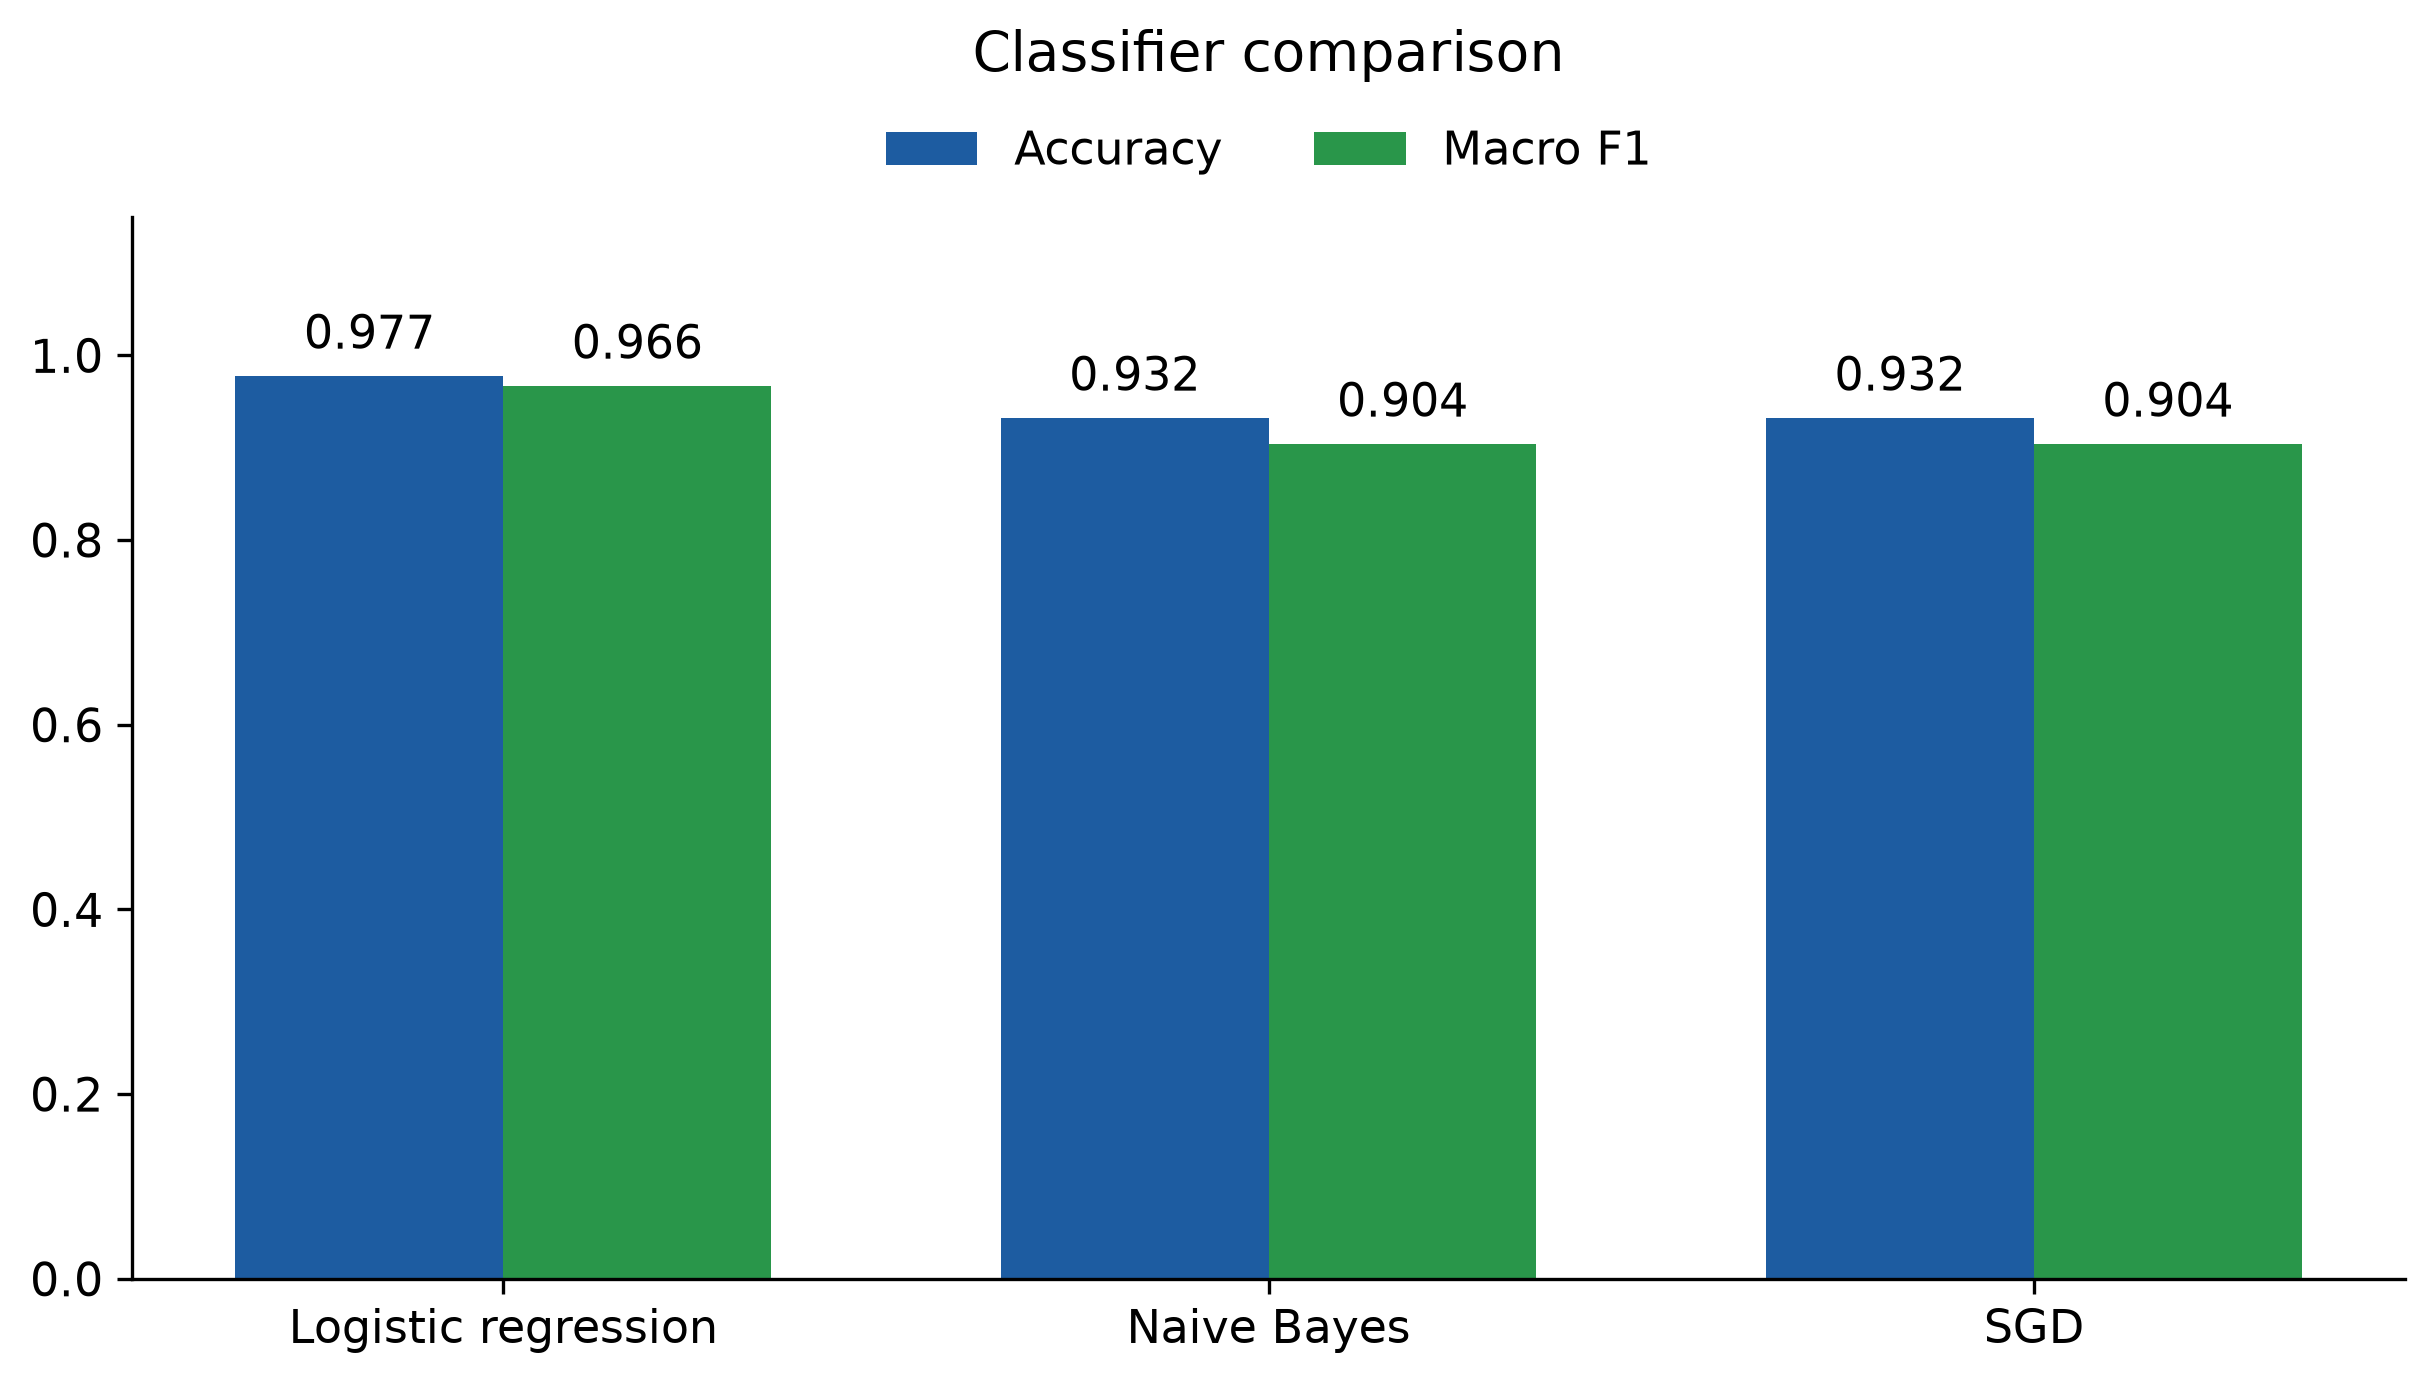
\includegraphics[width=\columnwidth]{Evaluation/figures/classifier_comparison.png}
\caption{Classifier comparison using the same held-out emails.}
\label{fig:classifier_comparison}
\end{figure}

\begin{figure}[H]
\centering
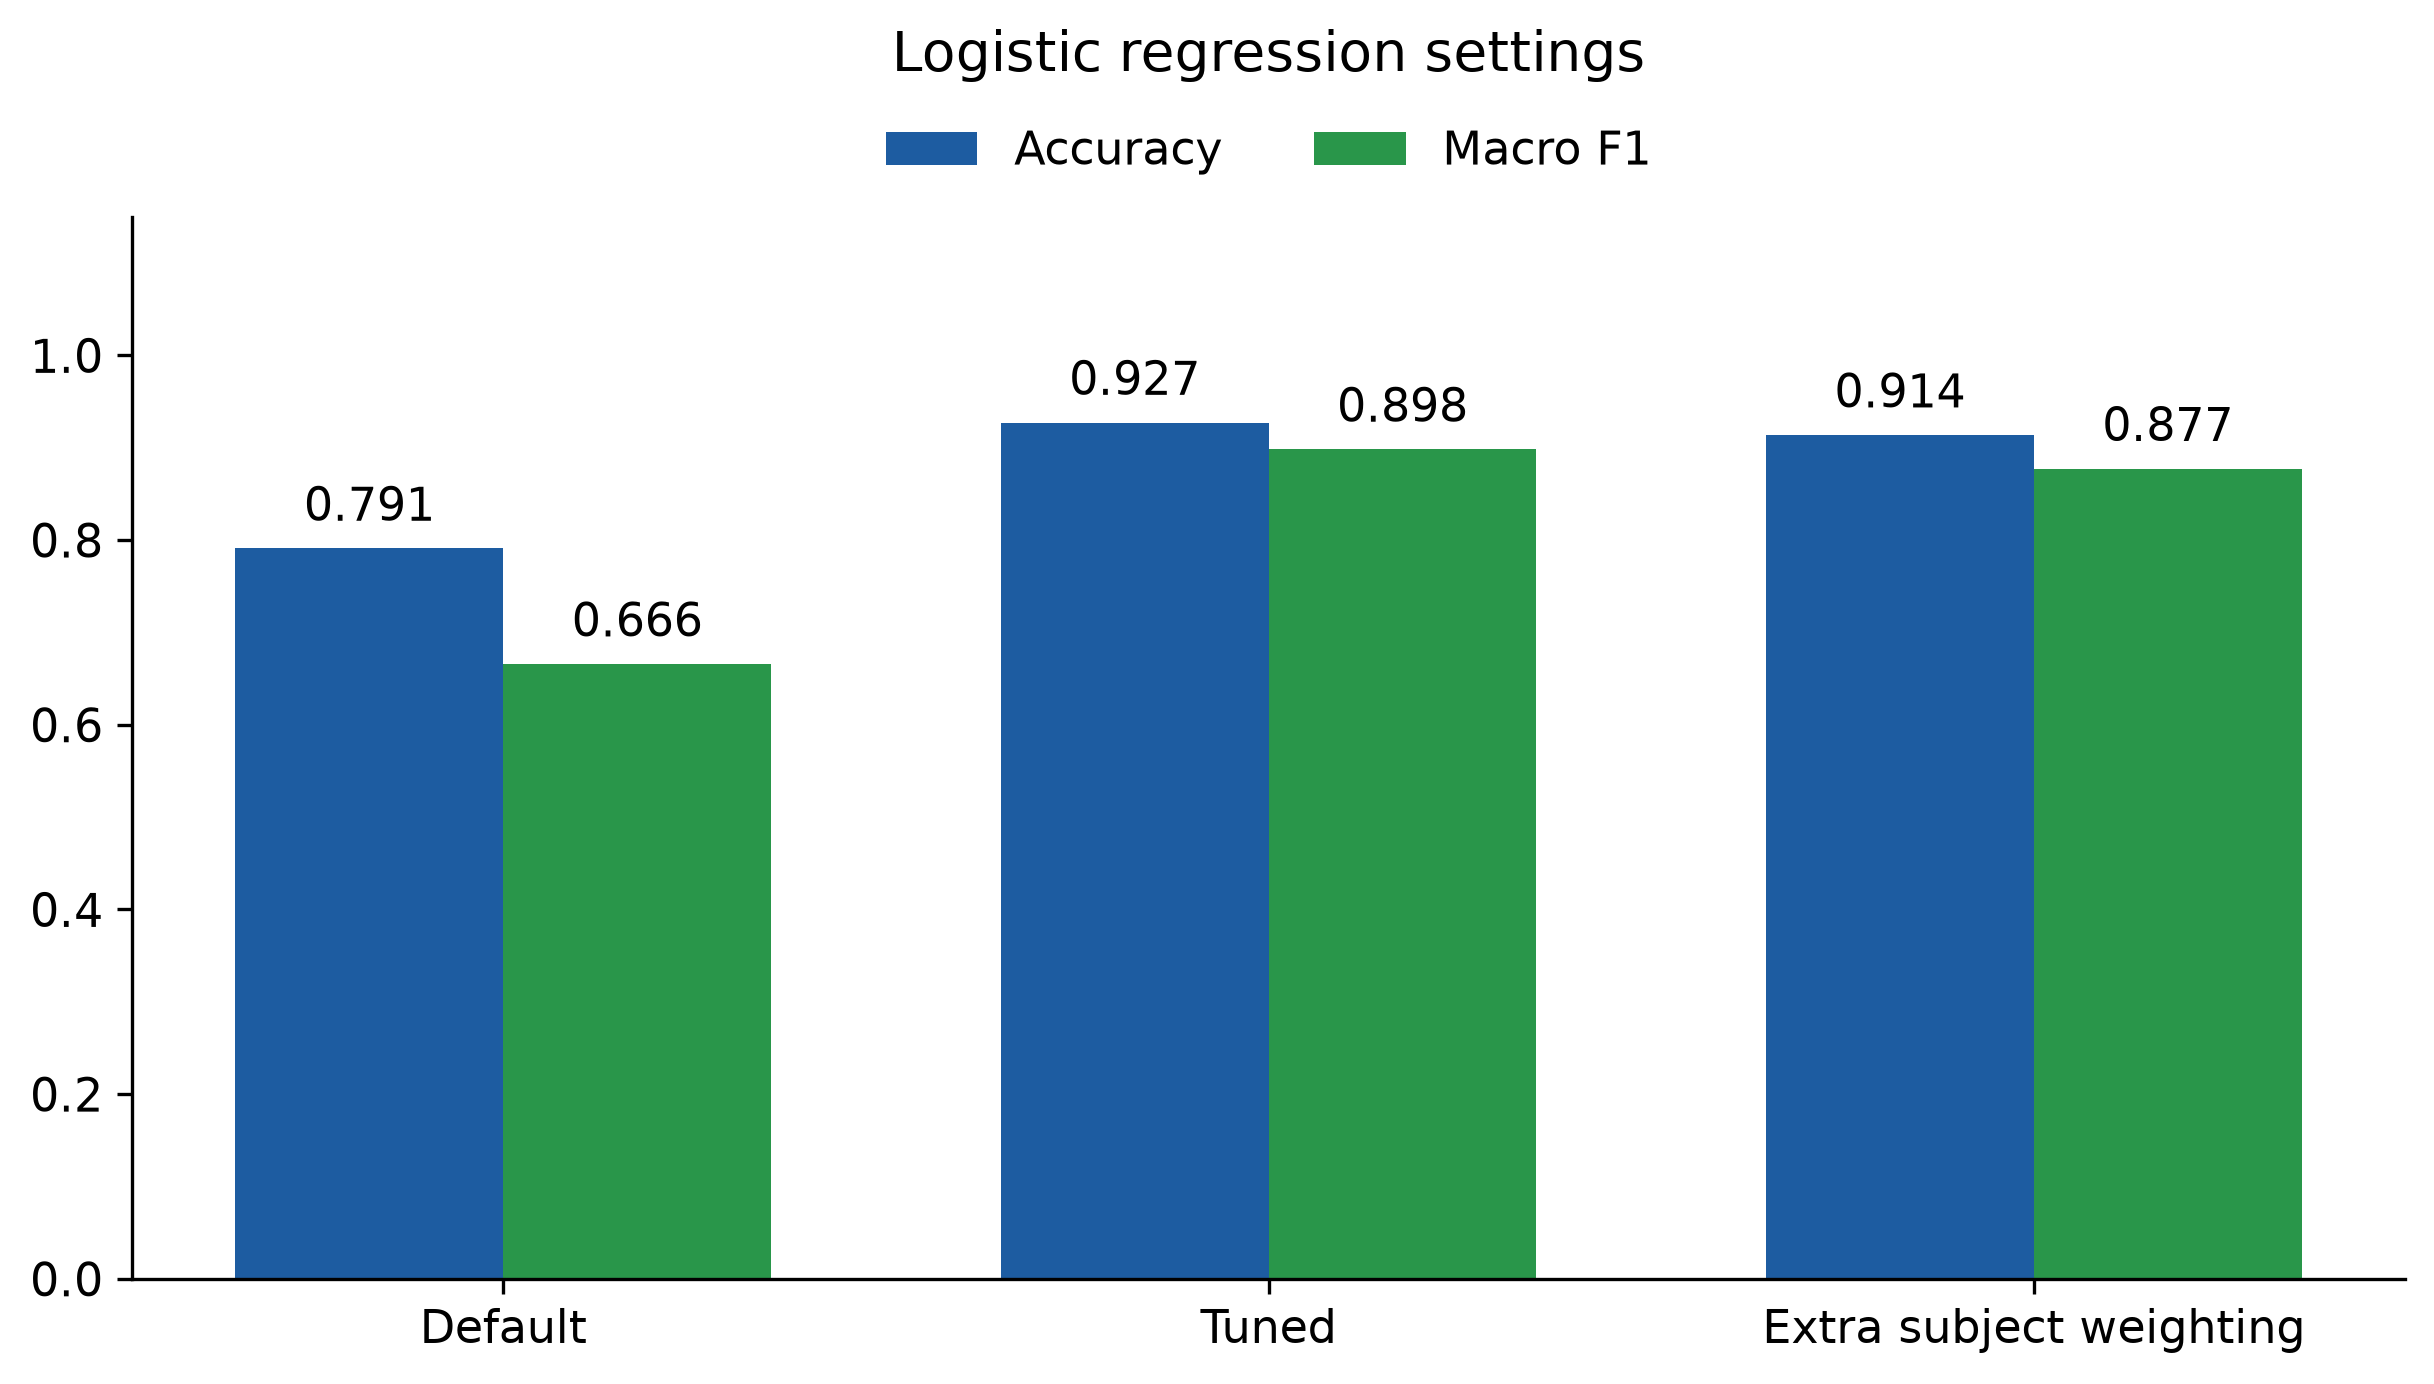
\includegraphics[width=\columnwidth]{Evaluation/figures/settings_comparison.png}
\caption{Mean cross-validation scores for the logistic regression versions.}
\label{fig:settings_comparison}
\end{figure}

\begin{figure}[H]
\centering
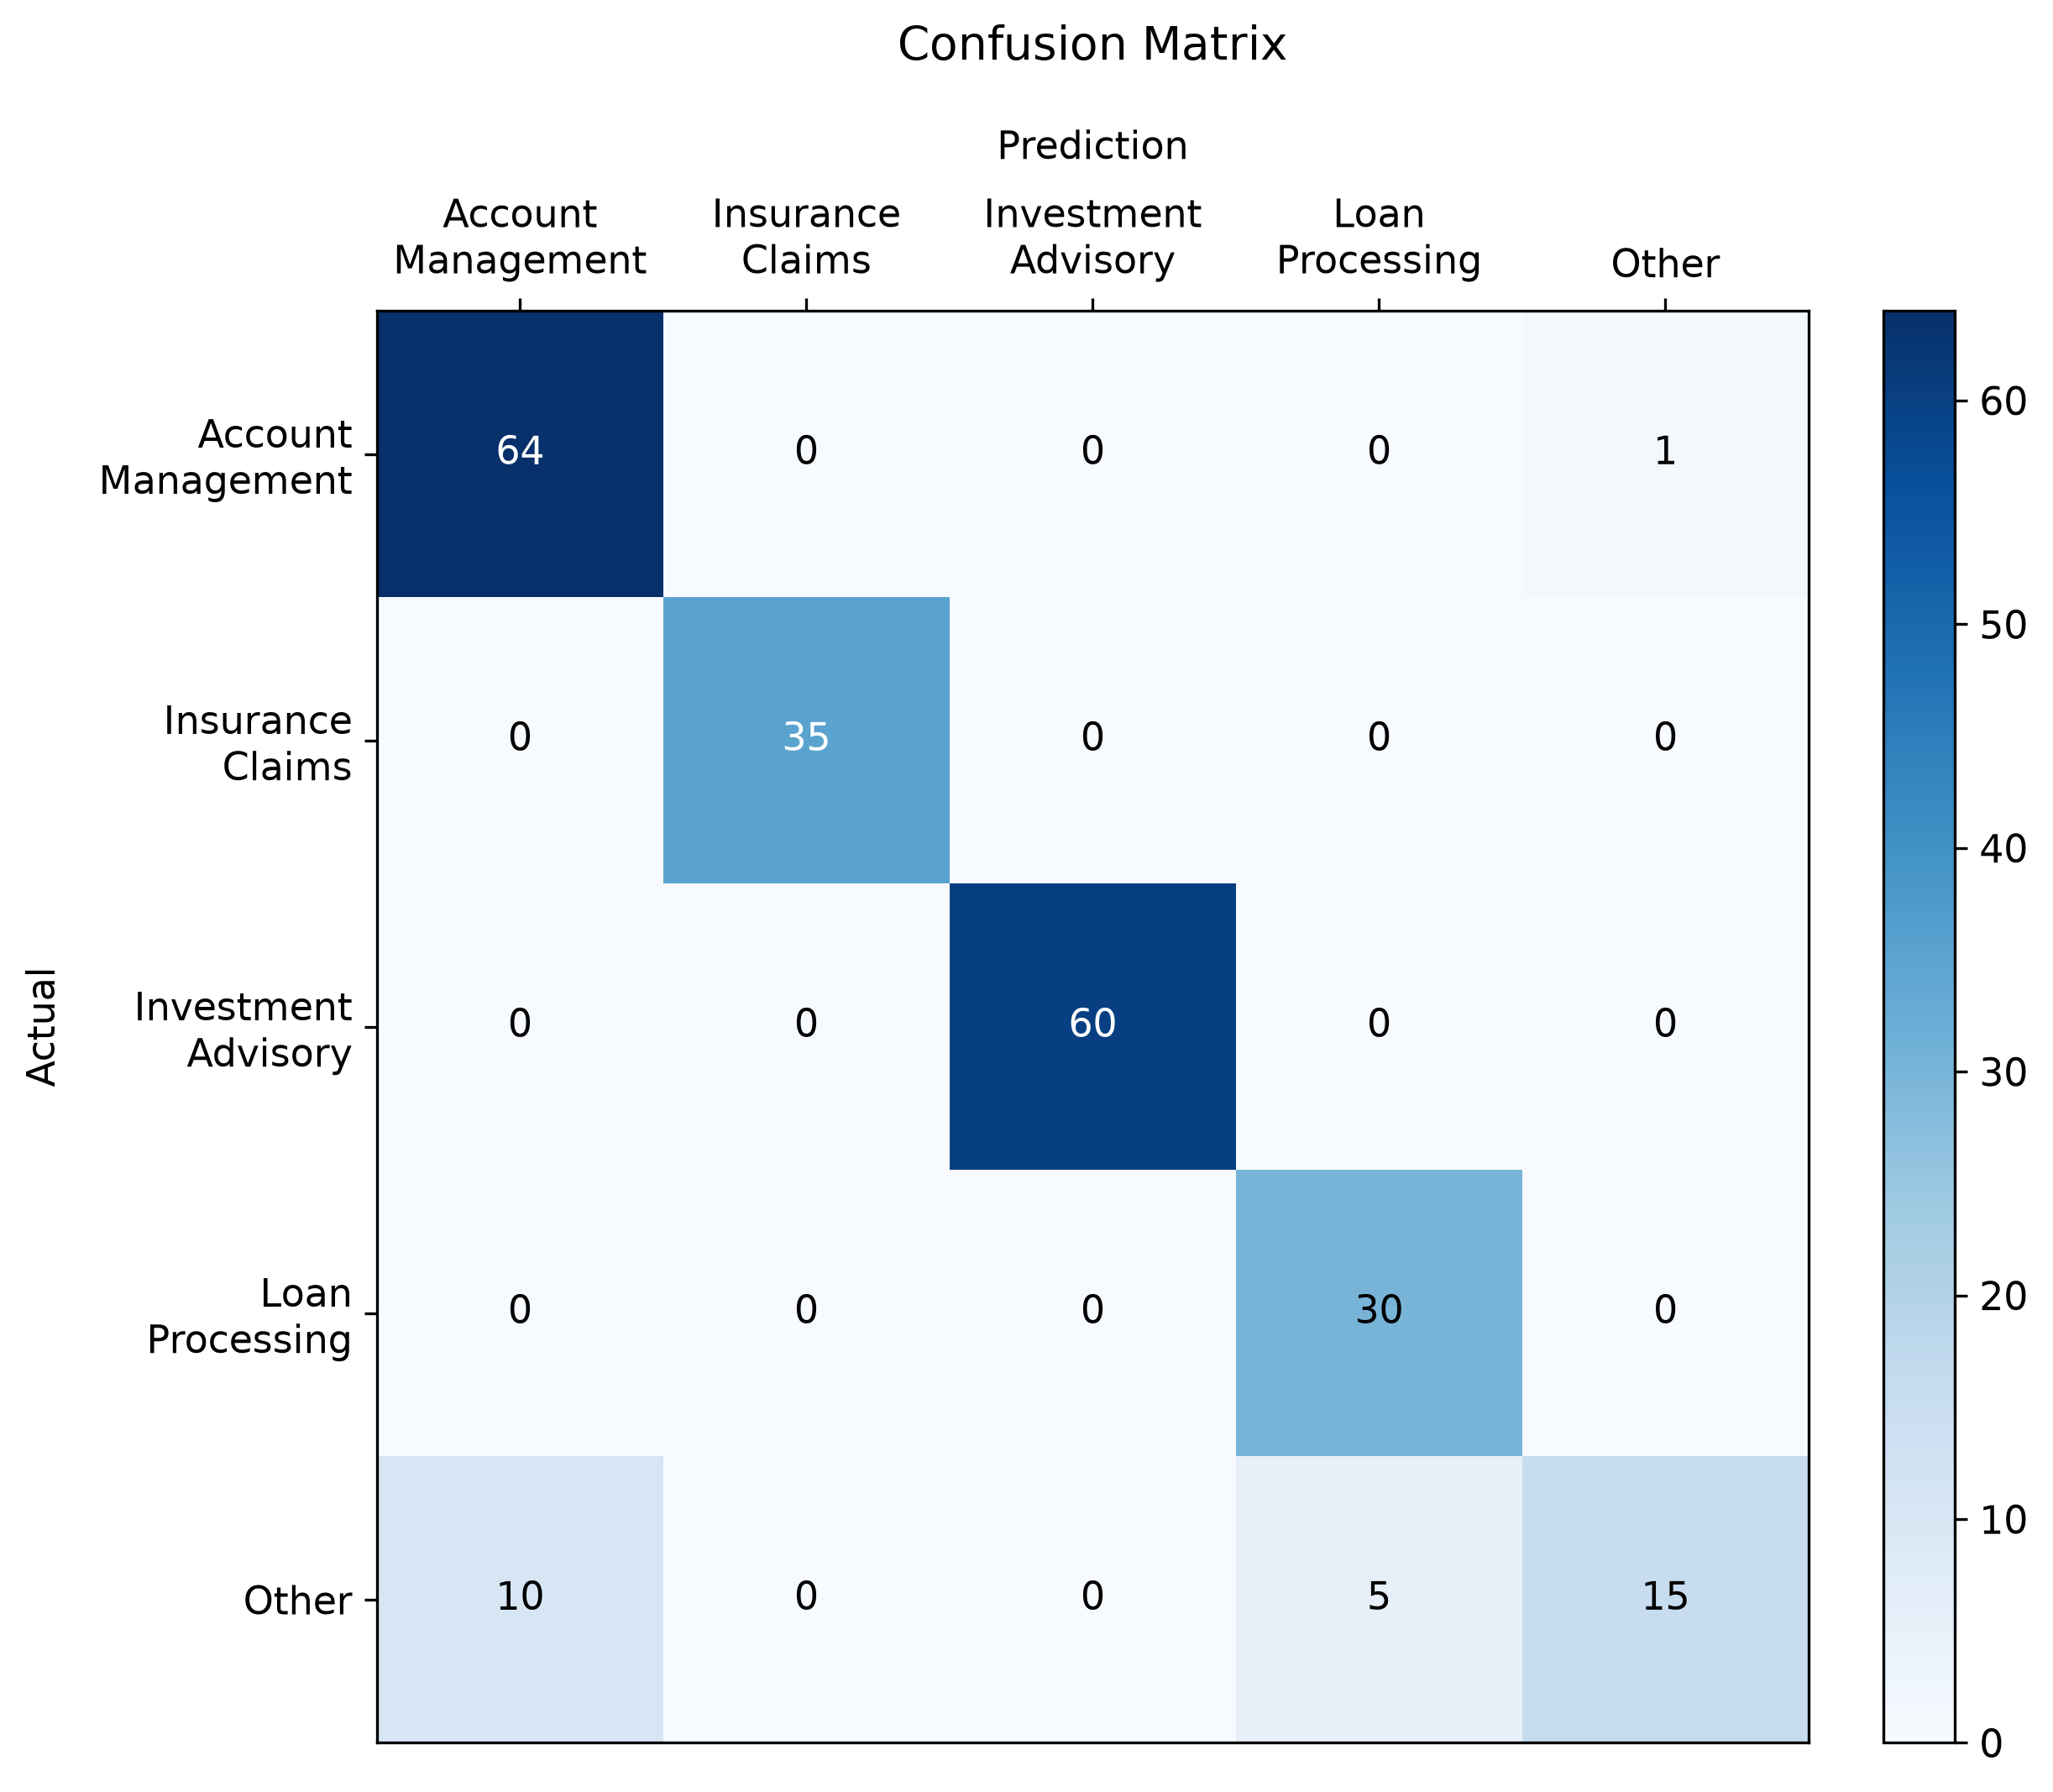
\includegraphics[width=\columnwidth]{Evaluation/figures/settings_tuned_matrix.png}
\caption{Tuned logistic regression confusion matrix. Counts combine five evaluations of each of the 44 labelled emails.}
\label{fig:settings_tuned_matrix}
\end{figure}

\begin{figure}[H]
\centering
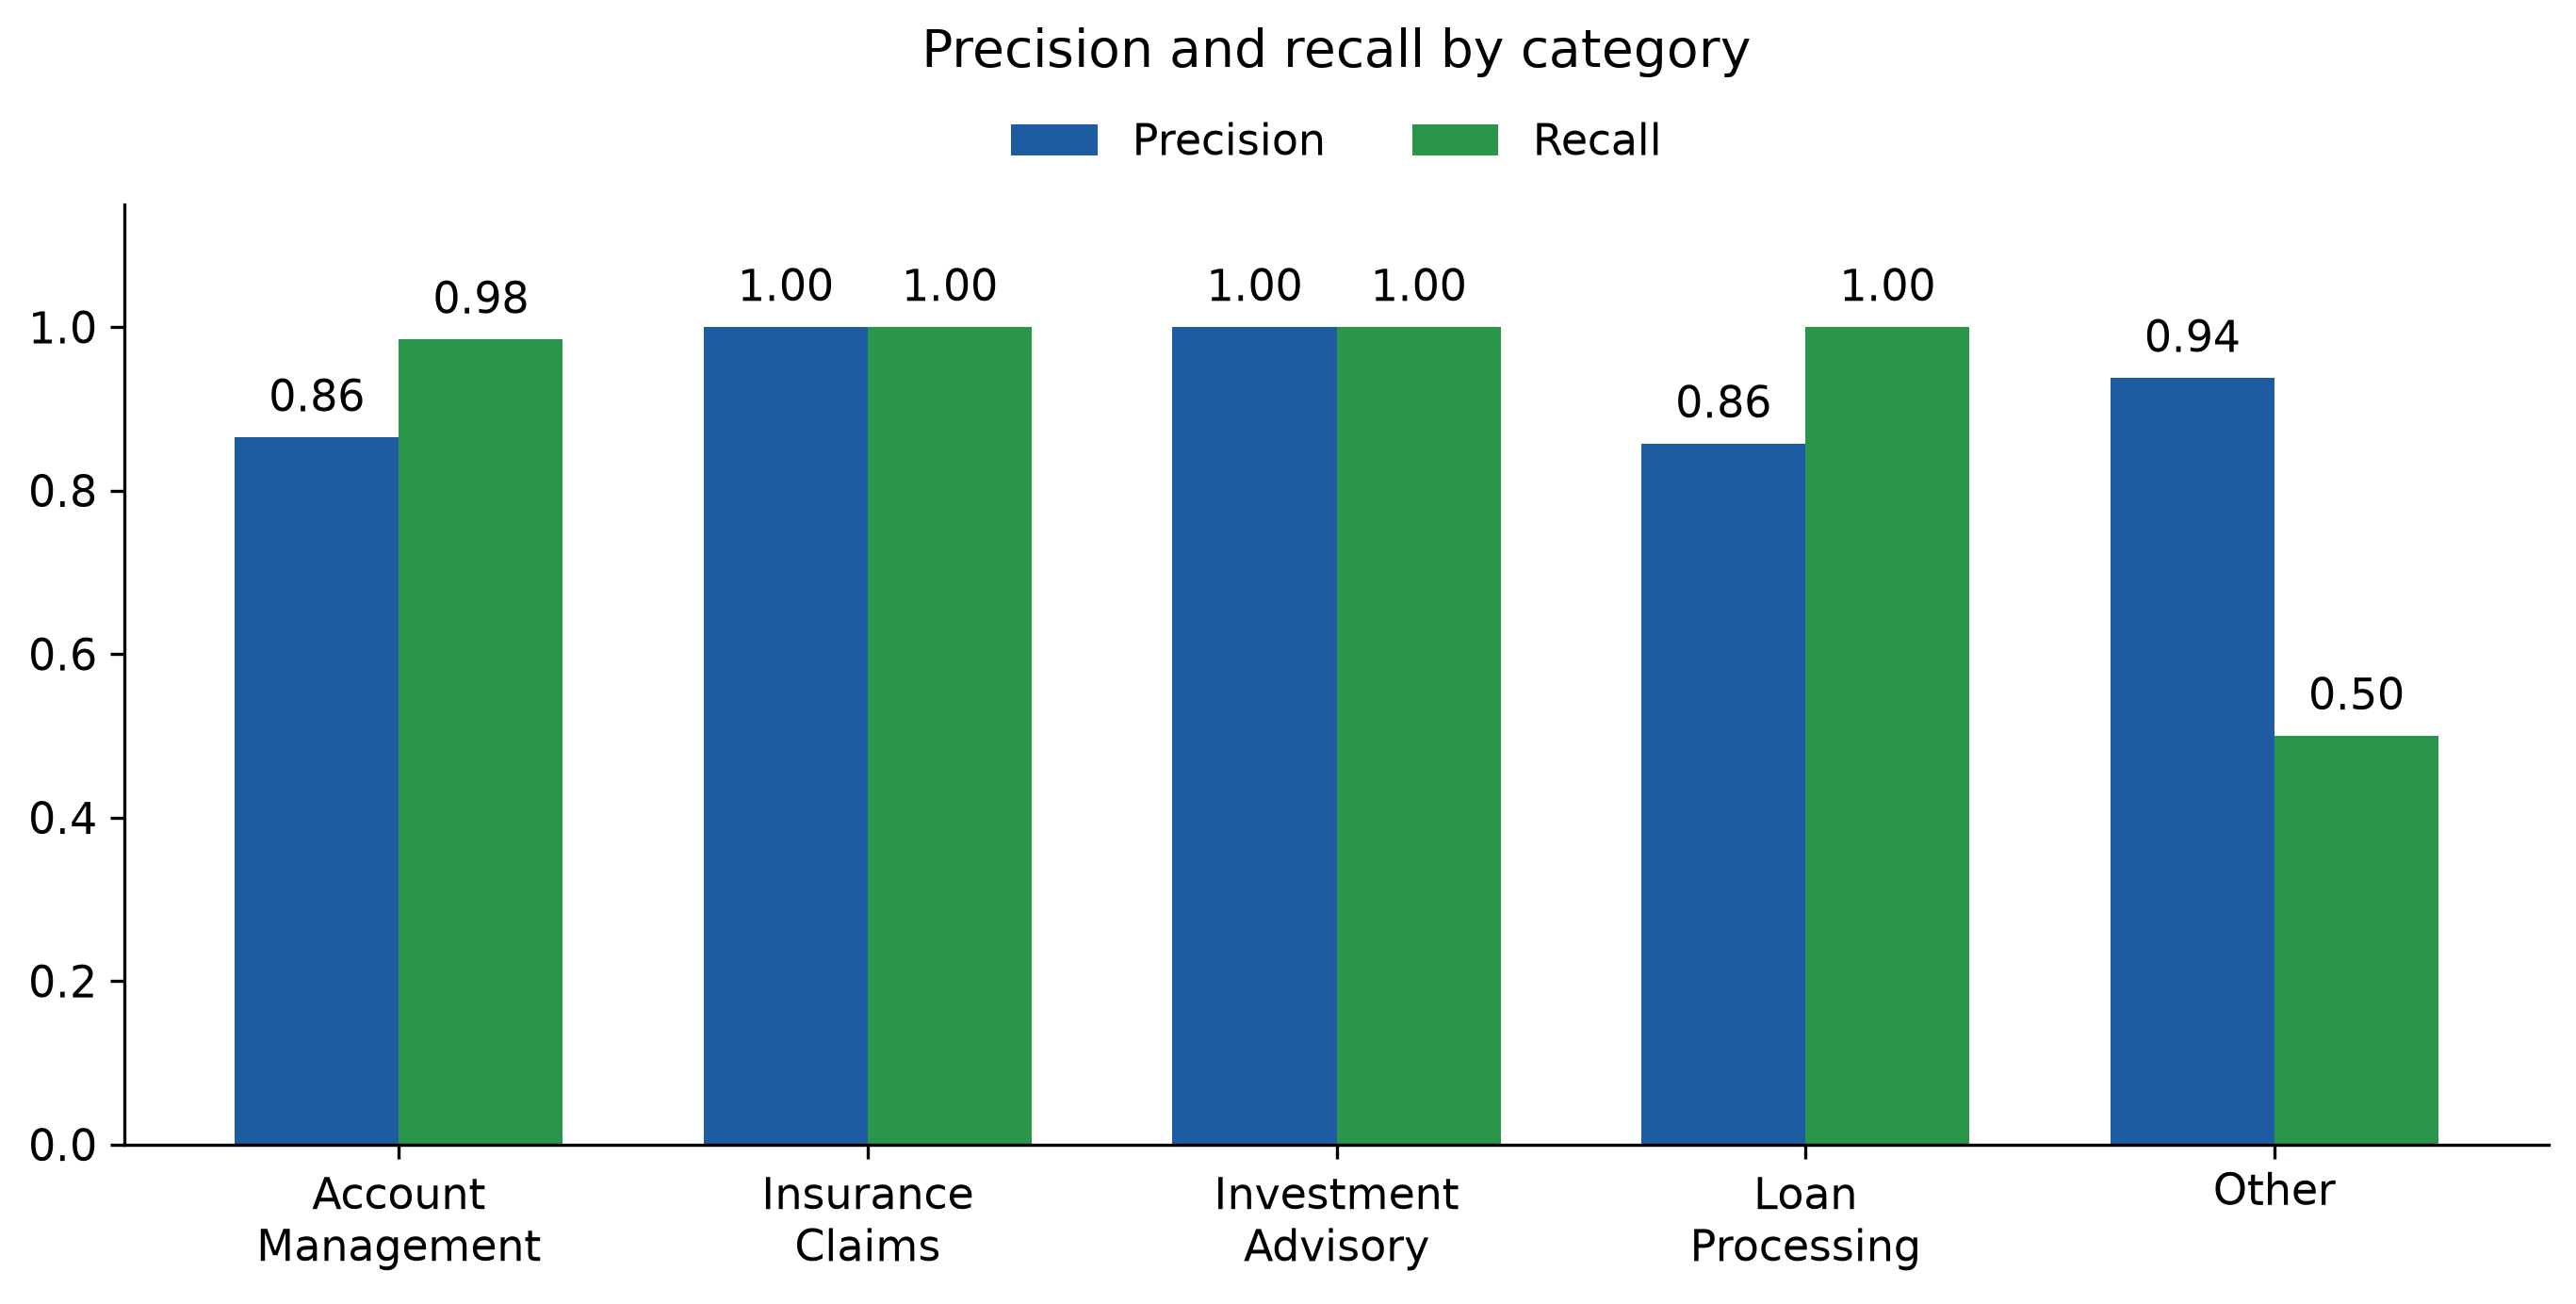
\includegraphics[width=\columnwidth]{Evaluation/figures/category_precision_recall.png}
\caption{Precision and recall by category for tuned logistic regression, calculated from pooled repeated cross-validation predictions.}
\label{fig:category_precision_recall}
\end{figure}

\end{document}
